%%
%% This is file `sample-acmlarge.tex',
%% generated with the docstrip utility.
%%
%% The original source files were:
%%
%% samples.dtx  (with options: `acmlarge')
%% 
%% IMPORTANT NOTICE:
%% 
%% For the copyright see the source file.
%% 
%% Any modified versions of this file must be renamed
%% with new filenames distinct from sample-acmlarge.tex.
%% 
%% For distribution of the original source see the terms
%% for copying and modification in the file samples.dtx.
%% 
%% This generated file may be distributed as long as the
%% original source files, as listed above, are part of the
%% same distribution. (The sources need not necessarily be
%% in the same archive or directory.)
%%
%%
%% Commands for TeXCount
%TC:macro \cite [option:text,text]
%TC:macro \citep [option:text,text]
%TC:macro \citet [option:text,text]
%TC:envir table 0 1
%TC:envir table* 0 1
%TC:envir tabular [ignore] word
%TC:envir displaymath 0 word
%TC:envir math 0 word
%TC:envir comment 0 0
%%
%%
%% The first command in your LaTeX source must be the \documentclass command.
\documentclass[acmlarge]{acmart}

\usepackage{tikz}
\usetikzlibrary{automata,positioning}
\tikzset{
    state/.style={
           rectangle,
           rounded corners,
           draw=black, very thick,
           minimum height=2em,
           inner sep=2pt,
           text centered,
           },
}
%%ss[STYLE]{acmart}
%% \BibTeX command to typeset BibTeX logo in the docs
\AtBeginDocument{%
  \providecommand\BibTeX{{%
    \normalfont B\kern-0.5em{\scshape i\kern-0.25em b}\kern-0.8em\TeX}}}
%% Rights management information.  This information is sent to you
%% when you complete the rights form.  These commands have SAMPLE
%% values in them; it is your responsibility as an author to replace
%% the commands and values with those provided to you when you
%% complete the rights form.
\setcopyright{acmcopyright}
\copyrightyear{2022}
\acmYear{2022}
\acmDOI{}


%%
%% These commands are for a JOURNAL article.
\acmJournal{POMACS}
\acmVolume{37}
\acmNumber{4}
\acmArticle{2}
\acmMonth{8}

%%
%% Submission ID.
%% Use this when submitting an article to a sponsored event. You'll
%% receive a unique submission ID from the organizers
%% of the event, and this ID should be used as the parameter to this command.
%%\acmSubmissionID{123-A56-BU3}

%%
%% The majority of ACM publications use numbered citations and
%% references.  The command \citestyle{authoryear} switches to the
%% "author year" style.
%%
%% If you are preparing content for an event
%% sponsored by ACM SIGGRAPH, you must use the "author year" style of
%% citations and references.
%% Uncommenting
%% the next command will enable that style.
%%\citestyle{acmauthoryear}

%%
%% end of the preamble, start of the body of the document source.
\begin{document}

%%
%% The "title" command has an optional parameter,
%% allowing the author to define a "short title" to be used in page headers.
\title{Paper Reading of \textit{Distributed snapshots: determining global states of distributed systems}}

%%
%% The "author" command and its associated commands are used to define
%% the authors and their affiliations.
%% Of note is the shared affiliation of the first two authors, and the
%% "authornote" and "authornotemark" commands
%% used to denote shared contribution to the research.
\author{Yiwei Yang}
\email{yangyw@shanghaitech.edu.cn}
\orcid{0000-0001-8011-5868}
\affiliation{
  \institution{ShanghaiTech University}
  \streetaddress{1 R.D. Zhongke}
  \city{Shanghai}
  \state{Shanghai}
  \country{China}
  \postcode{21210}
}

%%
%% By default, the full list of authors will be used in the page
%% headers. Often, this list is too long, and will overlap
%% other information printed in the page headers. This command allows
%% the author to define a more concise list
%% of authors' names for this purpose.
\renewcommand{\shortauthors}{Yiwei Yang}

%%
%% The abstract is a short summary of the work to be presented in the
%% article.
\begin{abstract}
  Many problems \cite{chandy1985distributed} in distributed systems can be attributed to the problem of obtaining global states, e.g. stable property detection, where a stable property is immutable, e.g., a computation has stopped or completed (which does not recover itself), a system deadlock (which does not recover itself), and through global states, these stable properties can be detected.
  For a distributed system, we need to record the global state of the system at the same point in time, including the state of each process and the state of the associated channel (a computation is a graph consisting of a finite number of processes and channels composed graph). This is the problem that the distributed snapshot algorithm solves, because there is no global unified lock, so it is impossible to guarantee that all processes can record their state information at the same time.
\end{abstract}

%%
%% The code below is generated by the tool at http://dl.acm.org/ccs.cfm.
%% Please copy and paste the code instead of the example below.
%%
\begin{CCSXML}
  <ccs2012>
  <concept>
  <concept_id>10010520.10010553.10010562</concept_id>
  <concept_desc>Computer systems organization~Embedded systems</concept_desc>
  <concept_significance>500</concept_significance>
  </concept>
  <concept>
  <concept_id>10010520.10010575.10010755</concept_id>
  <concept_desc>Computer systems organization~Redundancy</concept_desc>
  <concept_significance>300</concept_significance>
  </concept>
  <concept>
  <concept_id>10010520.10010553.10010554</concept_id>
  <concept_desc>Computer systems organization~Robotics</concept_desc>
  <concept_significance>100</concept_significance>
  </concept>
  <concept>
  <concept_id>10003033.10003083.10003095</concept_id>
  <concept_desc>Networks~Network reliability</concept_desc>
  <concept_significance>100</concept_significance>
  </concept>
  </ccs2012>
\end{CCSXML}

\ccsdesc[500]{Distributed System~Process Management}
\ccsdesc[300]{Concurrency~synchronization}

%%
%% Keywords. The author(s) should pick words that accurately describe
%% the work being presented. Separate the keywords with commas.
\keywords{Distributed System, Global State}


%%
%% This command processes the author and affiliation and title
%% information and builds the first part of the formatted document.
\maketitle

\section{Strong Point of the paper}
\subsection{The paper proposed Distributed snapshot algorithm}
A distributed system contains a finite set of processes and a finite set of channels, which can be described by a directed graph (vertices represent processes, edges represent channels), as shown in the following figure.

\begin{figure}[h]
  \centering
  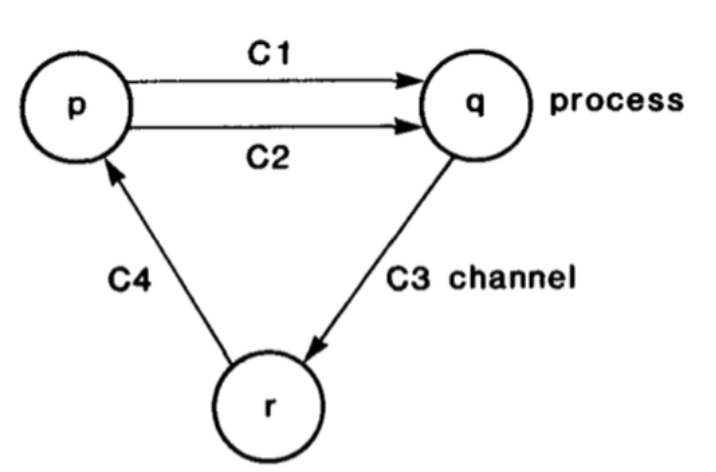
\includegraphics[width=0.3\linewidth]{./distributed_graph.png}
  \caption{Basic Model of Global State}
\end{figure}
\subsubsection{Two definitions}
\begin{enumerate}
  \item Channel: The article assumes that a channel has an infinite, zero-error, ordered buffer (and if not, whether the buffer is full), and that the delay of data in the channel is arbitrary and finite. The state of a channel is the msg list it has received upstream minus the msg list it has received downstream.
  \item Process: It is defined by a set of states, an initial state and a set of events. an event e in process p represents an atomic operation that may change the state of p itself and the state of the corresponding channel c (which may change its state when sending or receiving data).
\end{enumerate}
The event is defined as $<p, s, s^{\prime}, M, c>$, where
1. Process $\mathrm{p}$ is the place that event takes place;
2. The state before $e$'s state $\mathrm{p}$ is $s$
3. The state after $e$'s state $\mathrm{p}$ is $s^{\prime}$
4. Channel c's state will be changed by $e$
5. $M$ is the message send to or from $C$

\subsection{Global State Definitions}
With the previous model abstraction, here we can consider the global state of a distributed system as the set of process states and channel states. The initial global state is the set where each process is its corresponding initial state and each channel is the empty set.
An event $e$ may change the global state (here $s$), and another function is defined here: next $(S, e)$, which refers to the global state after the event $e$ occurs in the global state $s$, and according to the previous description, the global state after $e$ is processed The state of $\mathrm{p}$ is changed from $\mathrm{s}$ to $\mathrm{s}^{\prime}$, and the state of Channel $\mathrm{c}$ is added (data is sent to Channel $c$) or removed (data is sent away from Channel $c$) $m s g M$.
Here we define a $s e q=\left(e_{i}: 0 \leq i \leq n\right)$, which represents the sequence of events that will be processed by the distributed system, this seq is actually a computation of the system (this event sequence represents the distributed computation), assuming that before $e _{i}$ is processed, the global state of the system is $S_{i}$ (the initial state of the system is $S_{0}$), then the following equation can be obtained:
$$
S_{i+1}=\operatorname{next}\left(S_{i}, e_{i}\right), \text { for } 0 \leq i \leq n
$$
\subsection{Two Examples}
\subsubsection{Single-token Conservation}
In this system, there is a token that is transferred between two processes, and each process has two states: $s_0$ and $s_1$. If the process does not contain a token, its state is $s_0$, and if it contains a token, its state is $s_1$. p has an initial state of $s_1$ and q has an initial state of $s_1$. q's initial state is $s_0$. For each process, there are two types of event (here is an example to understand the previous concept of event, as shown in the diagram above).

When sending a token, the process state changes from $s_1$ to $s_0$.
When receiving a token, the process state changes from $s_0$ to $s_1$.
For the global state, there are four different possible states, as shown in the figure below.

\begin{figure}[h]
  \centering
  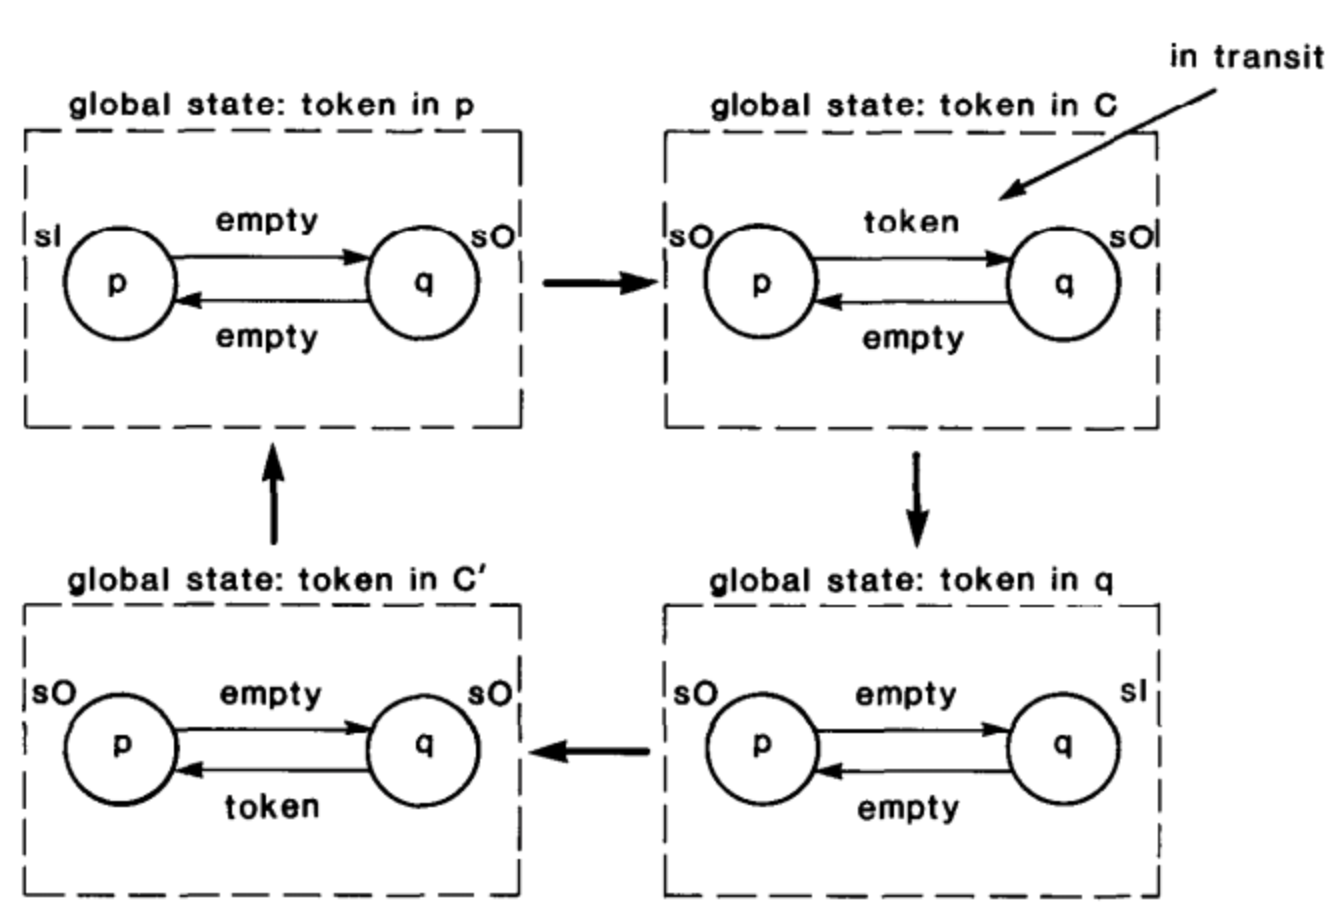
\includegraphics[width=\linewidth]{./single-token.png}
  \caption{Global states and transitions of the single-token conservation system.}
\end{figure}
\subsubsection{Non-deterministic computation}
For example, if two events, p sending M and q sending M', occur at the same time (the following is the case where these two events occur at the same time, as shown in the global state $S_2$ below), the resulting global state will be different from the expected one. The following diagram shows a possible global state transfer for this system.
\begin{figure}[h]
  \centering
  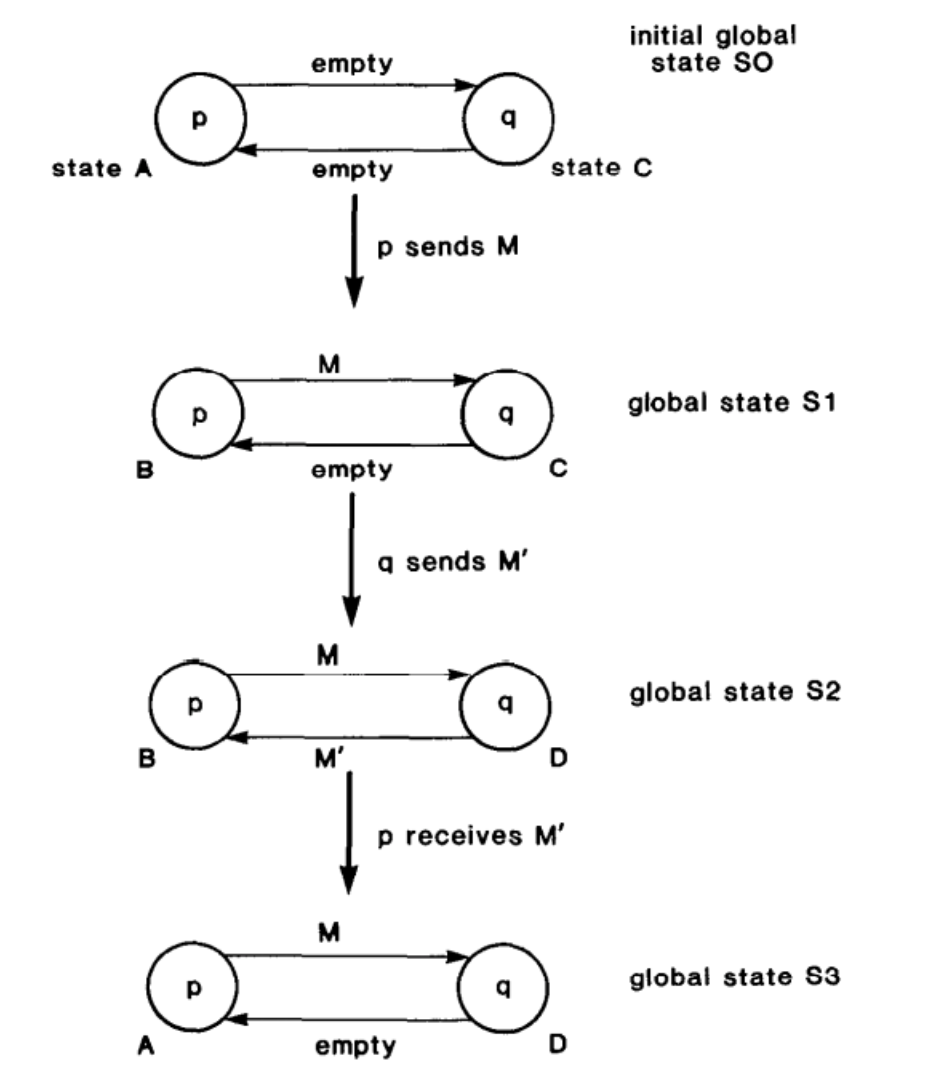
\includegraphics[width=0.4\linewidth]{./non-deterministic-comutation.png}
  \caption{Example for Non-deterministic computation}
\end{figure}
\subsubsection{Chandy-Lamport algorithm}
\begin{figure}[h]
  \centering
  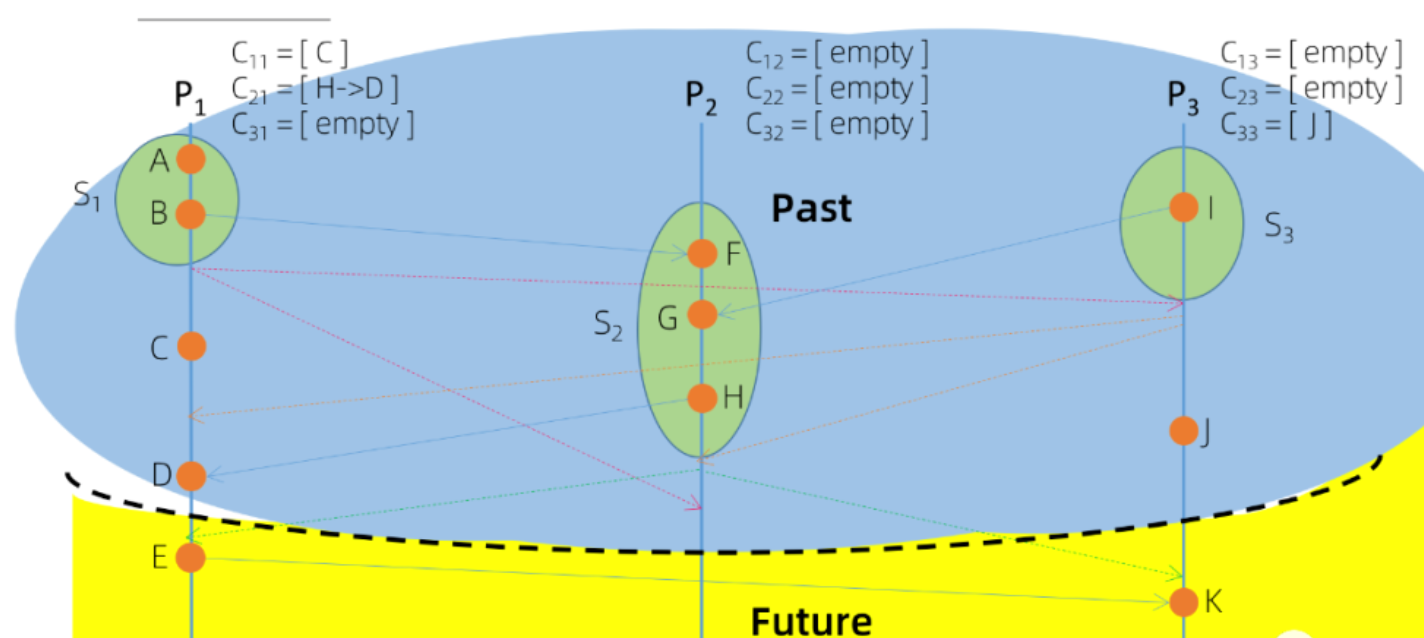
\includegraphics[width=\linewidth]{./chandy-lamport.png}
  \caption{Chandy-Lamport algorithm}
\end{figure}
\begin{enumerate}
  \item initiating a snapshot: a manager process (which is any of the processes) initiates a snapshot.
  \item manager process records process snapshot: the manager process starts recording its own local state (not including the state of the input channel), and after recording the local state, sends a marker to all downstream channels.
  \item manager process records channel snapshot: after the manager process takes its own snapshot, it records all input messages for each input channel until the marker message arrives, and then uses all messages during this period as a snapshot of this input channel.
  \item other processes record process snapshot: process starts recording process snapshot after it receives the first marker of all input channels upstream
  \item Other processes record channel snapshot: after the process takes its own snapshot, it records all the input messages for each input channel until the marker message arrives, and then takes all the messages during this period as the snapshot of this input channel (note that since this process has a input channel has already arrived, one of the input channel states recorded by this process will be empty).
  \item Terminate snapshot: After all processes have finished the local snapshot and channel snapshot, they send the finished message to the manager process, and after the manager process receives the message that all processes have finished the snapshot, the global consistency snapshot is finished.
  
\end{enumerate}
\section {Weak Point of the paper}
\subsection{The algorithm did not use vector clock algorithm}
Because at the time paper was proposed, the vector clock is not yet published, it was not used. By vector clock, the causal time will maintain the reverse property.
\subsection{The algorithm is the subset of Global Consistency Snapshot in flink \cite{carbone2015apache}}
It follows the following relationship:
\begin{center}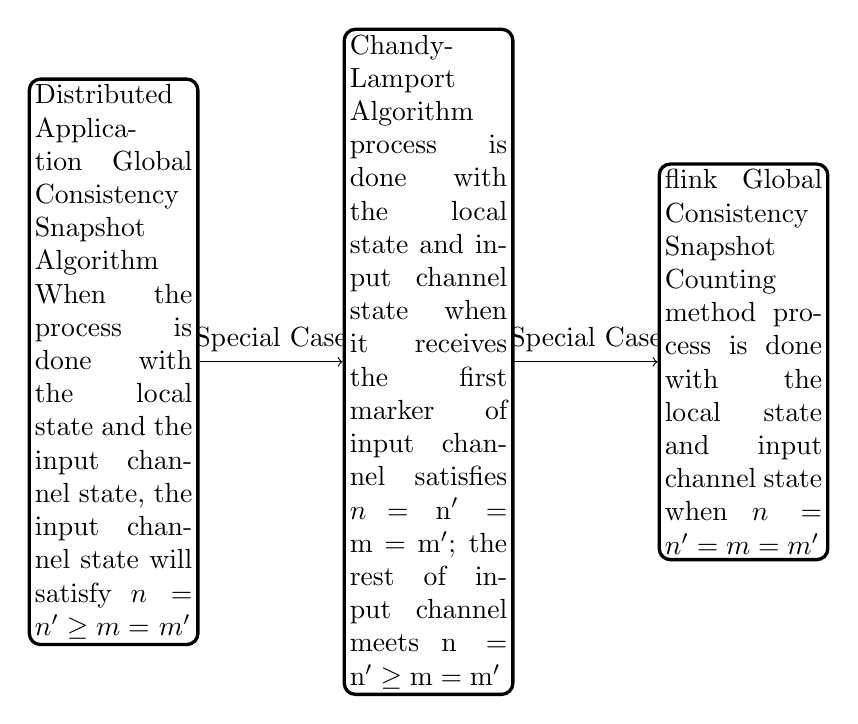
\begin{tikzpicture}
  \node[state] (I0) { 
    \parbox{2cm}{Distributed Application Global Consistency Snapshot Algorithm
    When the process is done with the local state and the input channel state, the input channel state will satisfy $n=n^{\prime} \geq m=$ $m^{\prime}$}
  };

  \node[state, right of=I0, node distance=4cm] (I2){
    \parbox{2cm}{Chandy-Lamport Algorithm
    process is done with the local state
    and input channel state
    when it receives the first marker
    of input channel satisfies $n$ $=\mathrm{n}^{\prime}=\mathrm{m}=\mathrm{m}^{\prime}$; the rest of
    input channel meets $\mathrm{n}=$
    $\mathrm{n}^{\prime} \geq \mathrm{m}=\mathrm{m}^{\prime}$}
  };		
  \node[state, right of=I2, node distance=4cm] (I1) { 
    \parbox{2cm}{flink Global Consistency Snapshot Counting
    method
    process is done with the local state
    and input channel state
    when $n=n^{\prime}=m=m^{\prime}$}
  };

  \path[->]
  (I0) 	edge 					node[above]{Special Case} (I2)
  (I2) 	edge 				 	node[above]{Special Case} (I1);

  
\end{tikzpicture}\end{center}
\section{Possible Refinement to the idea}
\subsection {The paper is not easy to implement}
The Chandy-Lamport algorithm describes a simple and straightforward but very effective distributed snapshot algorithm by abstracting the distributed system model. To discuss the Chandy-Lamport algorithm, it is important to note a few prerequisites of the algorithm: reliable network and orderly messages.

Spark's \cite{zaharia2010spark} Structured Streaming does not disclose more details about the Chandy-Lamport algorithm used to do Failover processing, although it is disclosed in the official blog. In contrast, Flink published a paper in 2015 \cite{carbone2015lightweight} that is more suitable for engineering implementation and has been applied in the Flink project. The core idea is to insert a barrier on the input source side to replace the Marker in the Chandy-Lamport algorithm, and to control the synchronization of the barrier to achieve backup and exactly-once semantics of snapshots. If you have read the Spark Streaming paper, one of the obvious questions about this area is how to handle stragglers (nodes that run significantly slower than other nodes in a distributed system), and the answer is that they cannot be handled.

\bibliographystyle{ACM-Reference-Format}
\bibliography{distributed_snapshots_determining_global_states_of_distributed_systems}


\end{document}
\endinput
%%
%% End of file `sample-acmlarge.tex'.
